\documentclass[10pt, a4paper]{article}
\usepackage[utf8]{inputenc}
\usepackage[T1]{fontenc,url}
\usepackage{multicol}
\usepackage{multirow}
\usepackage{parskip}
\usepackage{lmodern}
\usepackage{microtype}
\usepackage{verbatim}
\usepackage{amsmath, amssymb}
\usepackage{tikz}
\usepackage{physics}
\usepackage{mathtools}
\usepackage{algorithm}
\usepackage{algpseudocode}
\usepackage{listings}
\usepackage{enumerate}
\usepackage{graphicx}
\usepackage{float}
\usepackage{hyperref}
\usepackage{tabularx}
\usepackage{siunitx}
\usepackage{fancyvrb}
%\usepackage{natbib}
%\bibliographystyle{dinat}
\usepackage[makeroom]{cancel}
\usepackage[margin=2.0cm]{geometry}
\usepackage{pdfpages}
\usepackage[margin=10pt, textfont={small, it}, labelfont={bf}, labelsep=endash]{caption}
\renewcommand{\baselinestretch}{1}

\begin{document}
\title{COMAP - Vane angle vs TOD}
\author{
    \begin{tabular}{r l}
        Jonas Gahr Sturtzel Lunde & (\texttt{jonassl@astro.uio.no})
    \end{tabular}}
% \date{}    % if commented out, the date is set to the current date
\maketitle
Relevant code found at \url{https://github.com/jgslunde/comap_general/tree/master/vane_angle}
\vspace{0.7cm}


\begin{figure}[h!]
    \centering
    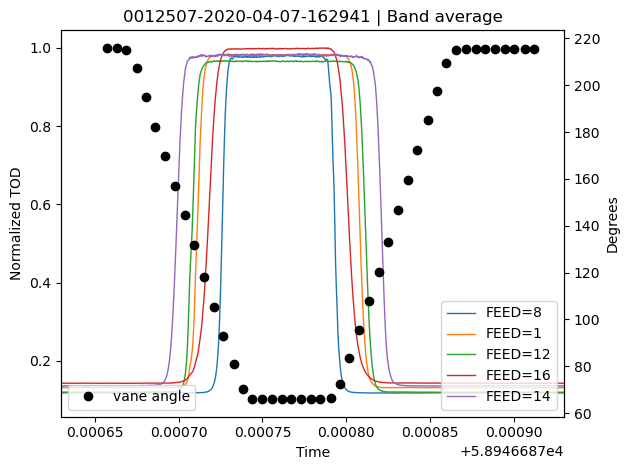
\includegraphics[scale=0.6]{../tod_angle.png}
    \caption{Normalized TOD power (thin lines) for a handful of feeds of a single level 1 file, together with vane angle (black dots) over a Tsys measurements. The TOD/angle relation should be completely symmetric in time, but a light offset can be seen (the TOD is seemingly lagging behind the vane angle). Another (expected) observed effect is the different widths of feeds TOD top hat, due to their differing physical placements on the feed array.}
    \label{fig:tod_angle}
\end{figure}


\begin{figure}[h!]
    \centering
    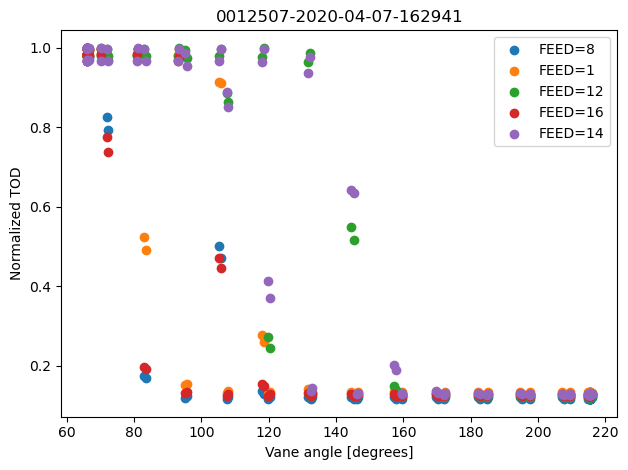
\includegraphics[scale=0.6]{../power_angle_single.png}
    \caption{Same setup as \ref{fig:tod_angle}. Normalized TOD power interpolated on and plotted against vane angle.}
    \label{fig:power_angle_single}
\end{figure}


\begin{figure}[h!]
    \centering
    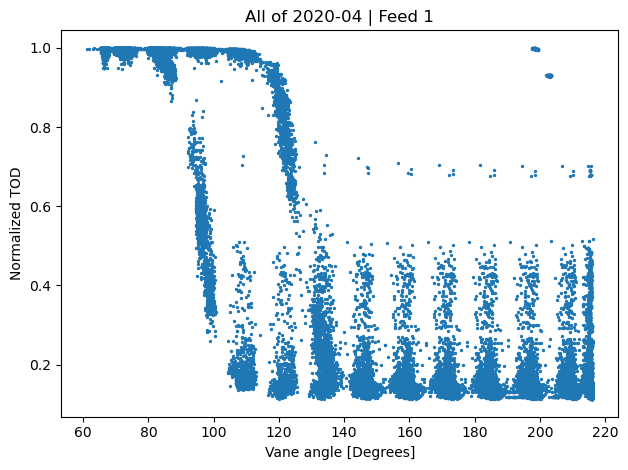
\includegraphics[scale=0.6]{../power_angle_all.png}
    \caption{Same type of plot as \ref{fig:power_angle_single}, but with all feed 1 obsids from 2020-04. We would expect the TOD/vane relation to be consistent between "vane descending" and "vane ascending", but we see two very distinct TOD/angle curves. This again strongly hints at an offset between the TOD and angle timestamps.}
    \label{}
\end{figure}


\begin{figure}[h!]
    \centering
    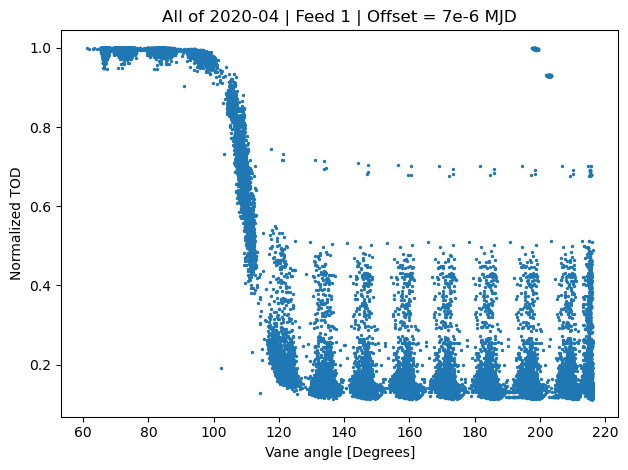
\includegraphics[scale=0.6]{../power_angle_all_7e-6.png}
    \caption{Introducing an offset of 7e-6 MJD (0.6 seconds) solves the problem, and gives us the plot like we expect it to look.}
    \label{}
\end{figure}


\begin{figure}[h!]
    \centering
    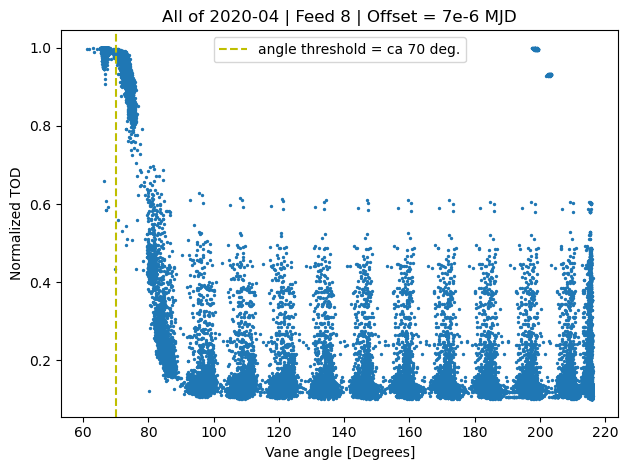
\includegraphics[scale=0.6]{../power_angle_all_feed8_7e-6.png}
    \caption{Same plot as above, but with feed 8, which is the farthest from the calibration vane, and therefore has the "worst" TOD/angle relation. We see that maximum power isn't reached until the vane as descended to at least 70 degrees.}
    \label{}
\end{figure}


\begin{figure}[h!]
    \centering
    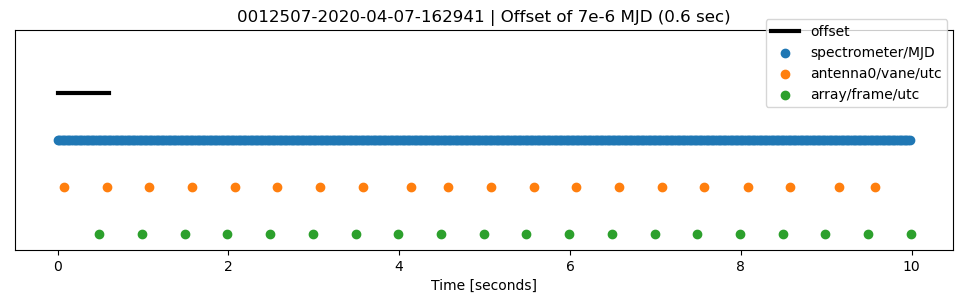
\includegraphics[scale=0.6]{../times_20.png}
    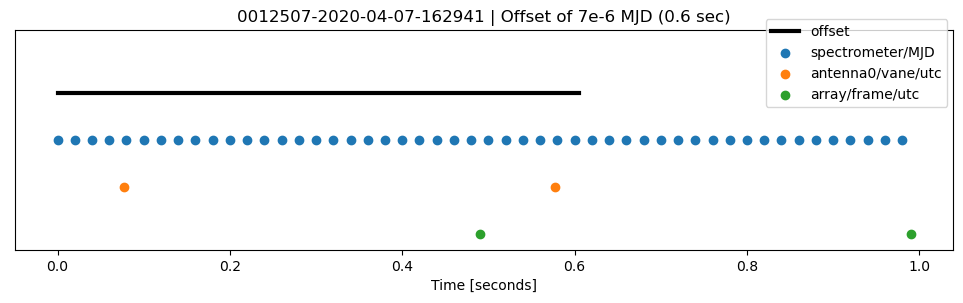
\includegraphics[scale=0.6]{../times_2.png}
    \caption{Plots showing the first 10 (above) and 1 (below) seconds of time stamps of the TOD, vane, and array. The offset we had to be introduced to get consistent results in previous plots is also shown, as a black line.}
    \label{}
\end{figure}



\end{document}